\documentclass[11pt,a4paper]{report}
\usepackage[latin1]{inputenc}
\usepackage{amsmath}
\usepackage{amsfonts}
\usepackage{amssymb}
\usepackage{graphicx}
\usepackage{url}
\usepackage{listings}
\usepackage{algorithm}
\usepackage{algpseudocode}

\author{He Xiao, Shijiao Yuwen}
\title{Prolog in Ocaml}
\begin{document}
	\maketitle
	
\begin{abstract}
	This report presents the design and implementation of the application `Prolog-Ocaml'.
	Basically, this project used Prolog \cite{PrologWiki} as a template, and designed a variant of Prolog in Ocaml;
	it covers the most basic phases of implementing a new programming paradigm: lexing, parsing, interpreting.
	Given the source code in predefined grammar, the delivered product can parse it to an internal AST and execute
	it. After testing it with some well-known Prolog programs and comparing the results with the official Prolog implementation,
	some strengths and weaknesses of our implementation have been found.  
\end{abstract}

\section*{Grammar}
There are several editions of prolog currently available online: SWI-prolog\cite{swi}, GNU-prolog\cite{gprolog}, Amzi-prolog\cite{amzi}, and so on. According to our research: they are not identical, including the grammar. The BNF grammar describing the acceptable input to our Prolog simulator is a core edition\cite{prologBNF} of the most basic prolog, so it is safe to start here.


\section*{Lexing and Parsing}
There are several editions of prolog currently available online: SWI-prolog\cite{swi}, GNU-prolog\cite{gprolog}, Amzi-prolog\cite{amzi}, and so on. They are not identical. When we were doing the literature review, we found an implementation of Amzi-prolog by Ocaml, but Amzi-prolog is more of an old fashion and its documentation are no longer available online. So our implementation is more close to SWI-prolog due to the better availability of reference. Because we are implementing a subset of prolog, only a subset of tokens are defined.
The overall layout and structure of lexer and parser in this project is the same as our mp homework. In lexer, we firstly define useful regular expressions, and then match symbols or regular expressions with corresponding tokens: there are independent entries for multi-line comments, single and double quoted string contents. In parser, we firstly define language tokens used by lexer and parser, and then the "goal" nonterminal of our grammar: we allow program entry parsing (with query) and rules entry parsing (without parsing), and finally we construct the stratification needed for unambiguous parsing with reference to the precedence table we found on SWI-prolog manual.



\begin{figure}
\centering
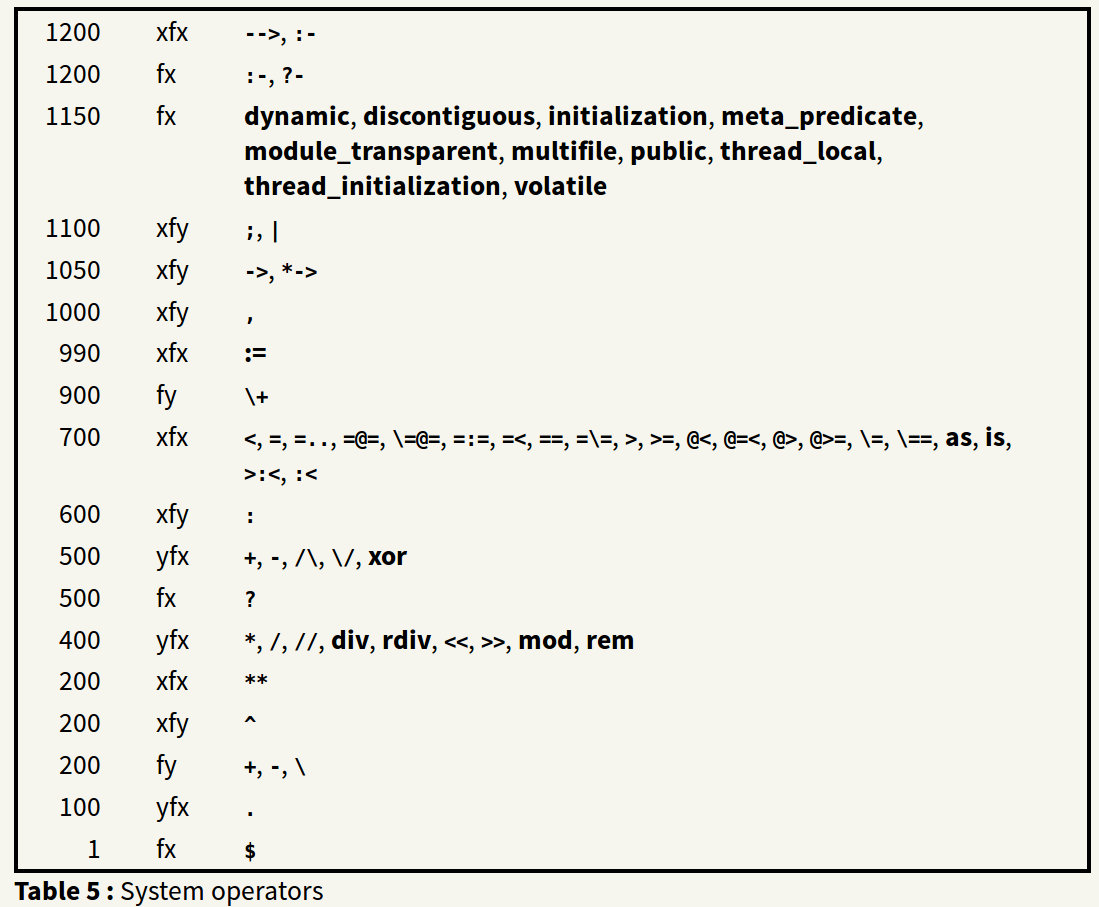
\includegraphics[width=0.9\linewidth]{precedenceTable}
\caption{Precedence table \cite{prologPrecedence}}
\label{fig:precedenceTable}
\end{figure}


\section*{Interpreting}
There are two preliminary functions involved in developing interpretation module. The first one is evaluation function for terms and the second one is for predicates.\\

In order to process the terms universally, a general value type is defined which covers all the primitive data types, namely `int', `float', `bool',`string',`list'. A constant term will be evaluated to its primitive value; A compound term which represents arithmetic operations or boolean logical operations will be simplified to a single value. A thing needs to be mentioned is that in standard Prolog, arithmetic operations like $+,-,*,/$ are overloaded, i.e. for both integer operations and floating point operations, the same operator symbol is used for each kind of operation. In order to handle this, both operands are converted to floating point numbers before doing computation if the two operands in a binary arithmetic operation have different precision levels. For $ListTerm$, each term inside the list will be evaluated and the values will be used to compose a value list. For variables terms, there is no way of evaluating an uninstantiated variable: there is no memory concept, variables are eliminated through substitution; as a result, if a variable is still a variable when doing the evaluation, it will never get any value and an exception will be thrown.
\bigskip
The other fundamental function is created for evaluating a predicate to either true or false. Again, the evaluation is performed through structural induction. At first, the predicate name will be checked, if it is one of the supported built-in function, then it will be interpreted in the `built-in' way. Interestingly, there exists an overlap between predicates and some proportion of compound terms: the binary boolean operators which return boolean values. For these things, their identities depend on the context in which they are evaluated. If the name of the predicate cannot be found in the built-in functions list, then the predicate will be passed to another function which will traverse the rules list to seek a match. In the case that some rule's head can be unified with the query predicate, then the body of the rule will be evaluated, and the final boolean result depends on the result of evaluating that body predicates. 

\bigskip
\subsection*{Algorithms For the Interpretation}

\begin{algorithm}
	\caption{Algorithm for evaluating a single predicate}
	
	\begin{algorithmic}
		\State Input: single predicate, rules
		\State Output: (true / false, substitution)
		
		\Function{eval\_predicate}{$rules$,$predicate$}
			\If{$predicate$ is built-in}
				\State evaluate $predicate$ accordingly
				\State \Return (evaluatedResult,[])
			
			\Else
				\State \Return EVAL\_PRED\_WITH\_RULES ($rules$, $predicate$)
			\EndIf
			
		\EndFunction
		
		\Function{eval\_pred\_with\_rules}{$rules$, $predicate$}
			\For{each clause $i$ in the rule list} 
				\If{$predicate$ unifiable with rule $i$'s head}
					\State get substitution $sigma$ from the unification
					\If {rule $i$ is a fact}
						\State \Return (true, $sigma$)	
						
					\Else
						\State Apply $sigma$ to the body of the rule (rename free vars if needed)
						\State Get the new query $q$
						\State Evaluate $q$ and get result $(b,sig2)$
						
						\If {$b$ is true}
							\State get final substitution $finalSig$ by composing $sig2$ and $sigma$
							\State \Return (true, $finalSig$)
							
						\Else
							\State continue, apply the next rule if possible
						\EndIf				
					\EndIf
				\EndIf
			\EndFor
			
			\State \Return (false,[])
		
		\EndFunction
		
	\end{algorithmic}
	
\end{algorithm}


\bigskip
Big picture:
Given a Prolog program consisting of a bunch of clauses and a query, our program is expected to
output the first result for the query, and its corresponding substitution. \\

Our application will first decompose the program to two parts: clause (either fact or rule) list and one query. Then decompose the Query to a list of predicates, where each individual predicate can be evaluated via the above algorithm. \\

The list of predicates in side the body part of a rule will be evaluated from left to right, and the list of predicates is left-associative. To help the computation of the final boolean result, a list of boolean connectives ($,$ or $;$ representing $\land$, $\lor$ respectively) is also provided by parser. Each time a predicate in the list obtains its result $(curBool,curSig)$, it will compute the new boolean value by applying the boolean operator (look up the top item in connective list) on the $lastBool$(the boolean result of previous predicate, which was computed by the last iteration) and $curBool$. After getting the $newBool$, it will pass it to the next iteration. The substitution $curSig$ will be used to update the remaining predicate list. \\

After getting the new boolean and new predicate list, the recursion can begin.

\section*{Backtracking}
Rigorously speaking, the backtracking algorithm implemented in this project is not the same as the classical ones. It will backtrack silently and try to
gather all the results, but it will not print the result immediately when find some; instead, it will output the results to the terminal after collecting all the results it obtains. In oder to simulate the behavior of standard Prolog, when multiple results are available, after presenting the first result, it will wait for the user's instruction and then respond accordingly.\\

Currently, in the application which uses backtracking algorithm (\textbf{play\_all.exe}), only Horn clause is supported: i.e. the body of the rules as well as the query must be predicates connected via logical and operators (in Prolog, `,').\\ Furthermore, in order to avoid entering infinite loops, a list is maintained which records, for each rule, all the queries that have matched the head predicate of that rule in the past. It has both advantages and disadvantages after adding this feature: the good thing is it will not get lost in one branch while some other results can be found easily in other branch; the bad thing is that it may have false alarm so that it will miss some true results. In the evaluation part, we will demonstrate that in certain area, the advantage of our approach outweigh its drawbacks.\\

\subsection*{Method for collecting all the results}
Each time a predicate is evaluated, even if a true result can be obtained in some path, it does not return immediately. Instead, it will continue using remaining rules to try to obtain other results. All these results are combined to form the final result list for evaluating the predicate.\\
To get all the results for a query with multiple predicates, the first predicate is first evaluated and we can get a list of results. For each result $(b,sig)$, we can use it to update the remaining predicate list and get a new query; then the result list for that branch can be obtained by consulting the updated query. The final result set is simply combining all the result lists in different branches. 


\section*{Testing Results and Evaluation}
In order to pass some certain tests, several built-in functions (such as `write', `nl' and most arithmetic and comparing functions) in Prolog are implemented, other than that, no built-in functions in Prolog are supported.\\

The output format is simulating Prolog's. If no result is found, then a $false$ will be given.
If multiple results are available, then the substitutions will be printed one by one if the user requires. If there is no substitution exists and the query succeeds, then a true will be given.

\subsection*{Factorial}
\begin{lstlisting}
	factorial(0,1). 
	factorial(N,F) :- 
	N>0, N1 is N-1, factorial(N1,F1),
	F is N * F1. 
	
	?- factorial(5,W).
\end{lstlisting}
Output:\\
$W=120.$


\subsection*{Hanoi}
\begin{lstlisting}
	 move(1,X,Y,_) :-  
	 write('Move top disk from '), 
	 write(X), 
	 write(' to '), 
	 write(Y), 
	 nl. 
	 move(N,X,Y,Z) :- 
	 N>1, 
	 M is N-1, 
	 move(M,X,Z,Y), 
	 move(1,X,Y,_), 
	 move(M,Z,Y,X).  
	 ?-  move(3,left,right,center). 
\end{lstlisting}

Output:
\begin{lstlisting}
	'Move top disk from 'left' to 'right
	'Move top disk from 'left' to 'center
	'Move top disk from 'right' to 'center
	'Move top disk from 'left' to 'right
	'Move top disk from 'center' to 'left
	'Move top disk from 'center' to 'right
	'Move top disk from 'left' to 'right
	
	true.
\end{lstlisting}

\subsection*{List Size}
\begin{lstlisting}
	size([],0).
	size([H|T],N) :- size(T,N1), N is N1+1.
	
	?- size([1,2,3,4],N).
	
	Output: 
	N=4.
\end{lstlisting}



\subsection*{Transitive relation}
\begin{lstlisting}
sis(joyce,niu).
sis(keke,joyce).
sis(joyce,ker).
sis(X,Y) :- sis(X,Z), sis(Z,Y).
?-sis(X,Y).
\end{lstlisting}

\begin{lstlisting}
	Output:
	X=joyce.
	Y=niu.
	;
	
	X=keke.
	Y=joyce.
	;
	
	X=joyce.
	Y=ker.
	;
	
	X=keke.
	Y=niu.
	;
	
	X=keke.
	Y=ker.
	
\end{lstlisting}

This transitive example is where our implementation achieves a better result than the official SWI-Prolog: the official Prolog only gets the results from the facts, but it runs out of its stack before getting the other two results via applying the last rule. 

\bigskip

\section*{Limitations}
\begin{itemize}
	\item In the implementation of the `play.exe' which retrieves a single result, a true result may not be found in the situation where a rule's head can unify with the predicate but the rule does not fire due to the body part does not return true. \\
	
	\item If the input argument is too large, then `play\_all.exe' may not compute the results correctly. Some incorrect result has been found when compute the factorial with big number.
	
	\item Some feature like $Cuts$ are not supported in the current implementation of our tool.
\end{itemize}

Due to the time constraints, the application is not tested thoroughly; but to the best of our knowledge, it runs as expected on the provided classic examples.


\section*{Possible future work}
\begin{itemize}
	\item Currently, not many built-in functions are supported due to the limited implementation time. However, an idea is that, given the path to official Prolog's library, if the built-in functions are also written in normal syntax of Prolog program, then our implementation should be able to make use of those built-in rules and obtain the results as if all the rules are defined locally in one file.
	
	\item Currently, due to the limitation of algorithms used, some results may not be detected even if they are true. An idea to solve this problem is by adding the results obtained from last query as facts to the knowledge base, so in the future queries, those previously missing results will not be missed again. This design is also reflecting the process of  human child's continuously learning via remembering facts. Another possible solution is: before returning the computed results to the user, the application can analyze the results and get some new facts and place them into the knowledge base. After that, the application re-run the query to check whether the new results obtained is the same as the previous one (if multiple results available, the order maybe different). This process is repeated until a fixed point is reached, when the final complete result will be returned to the user. 
\end{itemize}


\bibliographystyle{plain}
\bibliography{dblp}

\section*{Appendix}
\lstinputlisting[caption={Data Structures}, label={Types in Ocaml representing program constructs of Prolog}, firstline=2, lastline=27]{../projCommon.ml}

\end{document}
